\subsection{Multimeter light source plots}

\begin{figure}[H]
\begin{subfigure}[h]{0.50\textwidth}
        \centering
        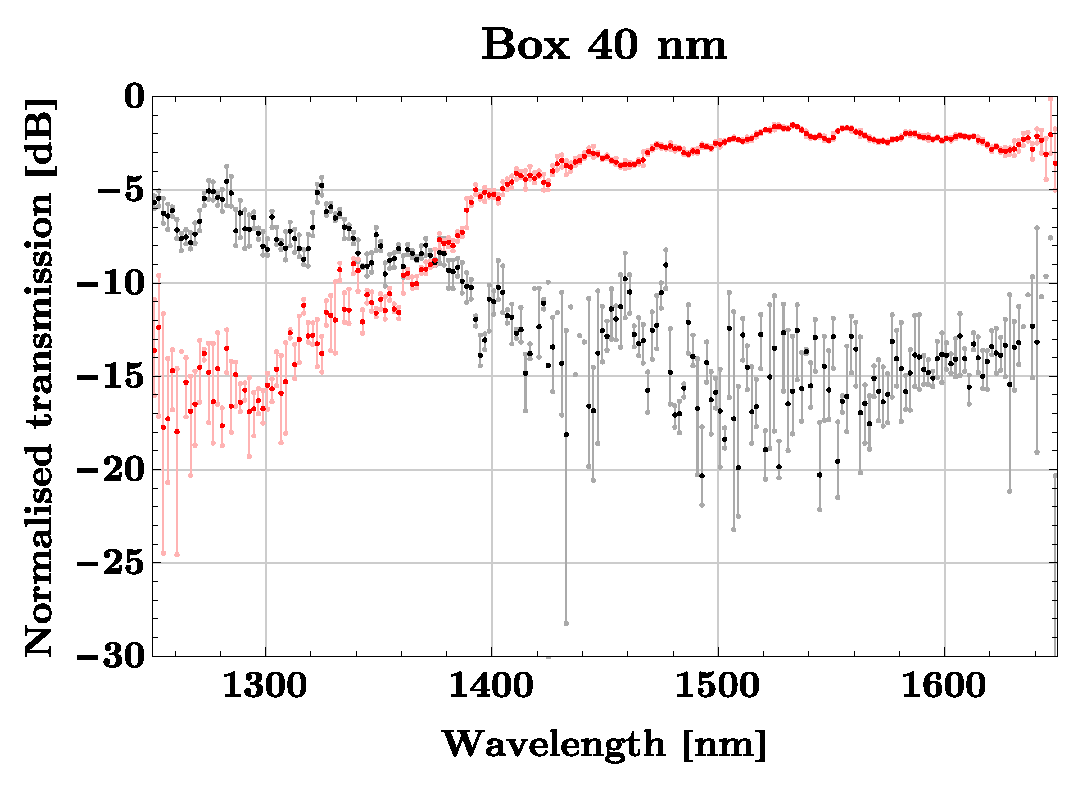
\includegraphics[width=1.0\textwidth]
        {fig/Kilde2Multimeter/box40multimeterconcatenated.eps}
        \caption{Transmission through the box structure with feature size 40 nm.}
    \end{subfigure}%
    ~ 
    \begin{subfigure}[h]{0.50\textwidth}
        \centering
        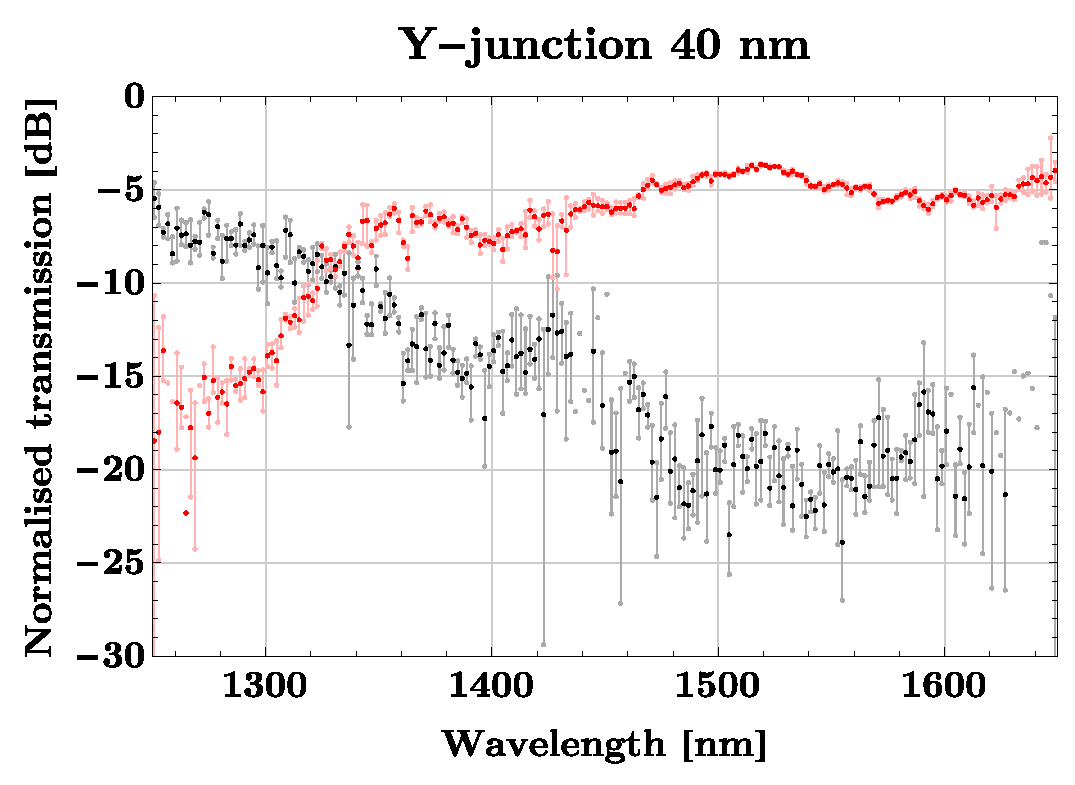
\includegraphics[width=1.0\textwidth]
        {fig/Kilde2Multimeter/yjunc40multimeterconcatenated.eps}
        \caption{Transmission through the Y-junction structure with feature size 40 nm.}
    \end{subfigure}
    
    \vspace{5 mm}
    
    
    \begin{subfigure}[h]{0.50\textwidth}
        \centering
        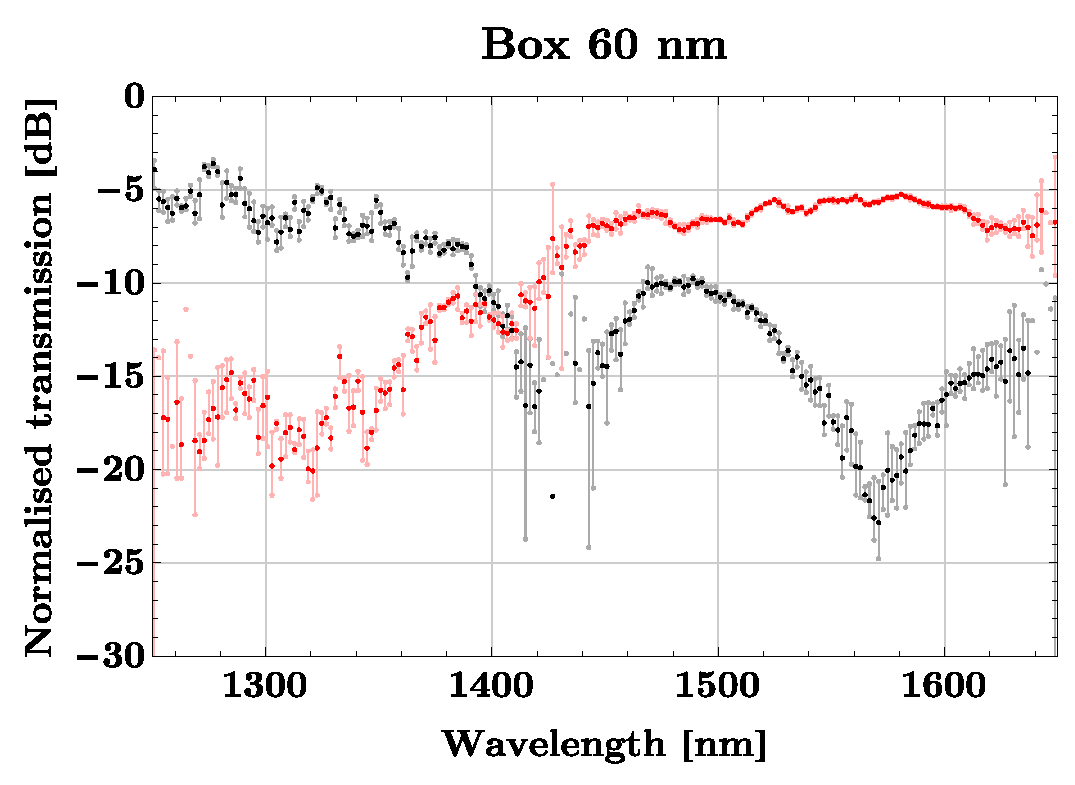
\includegraphics[width=1.0\textwidth]
        {fig/Kilde2Multimeter/box60multimeterconcatenated.eps}
        \caption{Transmission through the box structure with feature size 60 nm.}
    \end{subfigure}%
    ~ 
    \begin{subfigure}[h]{0.50\textwidth}
        \centering
        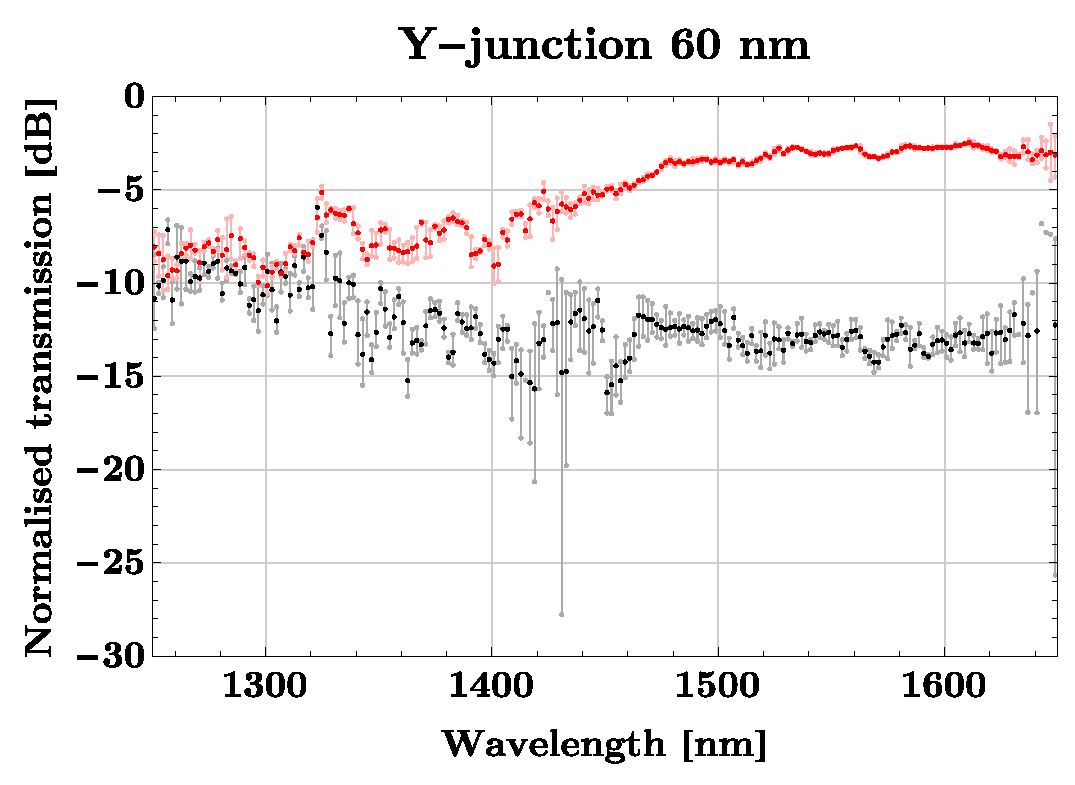
\includegraphics[width=1.0\textwidth]
        {fig/Kilde2Multimeter/yjunc60multimeterconcatenated.eps}
        \caption{Transmission through the Y-junction structure with feature size 60 nm.}
    \end{subfigure}
    
    \vspace{5 mm}
    
    \begin{subfigure}[h]{0.5\textwidth}
        \centering
        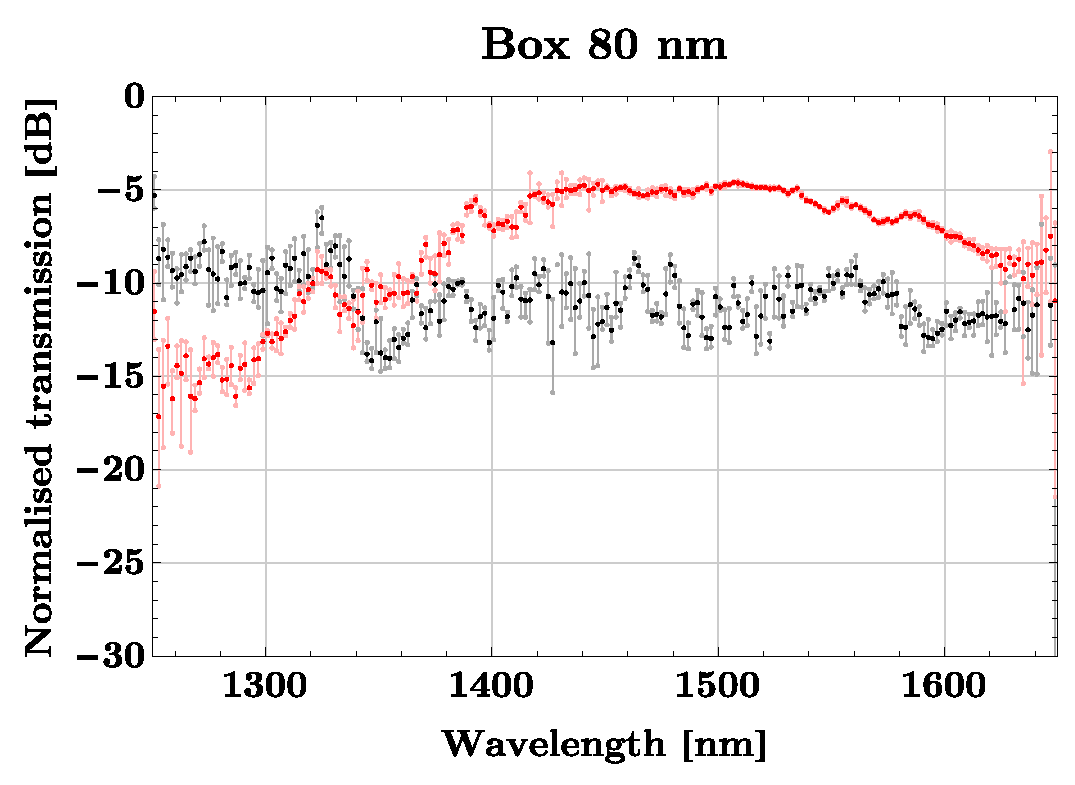
\includegraphics[width=1.0\textwidth]
        {fig/Kilde2Multimeter/box80multimeterconcatenated.eps}
        \caption{Transmission through the box structure with feature size 80 nm.}
    \end{subfigure}%
    ~ 
    \begin{subfigure}[h]{0.50\textwidth}
        \centering
        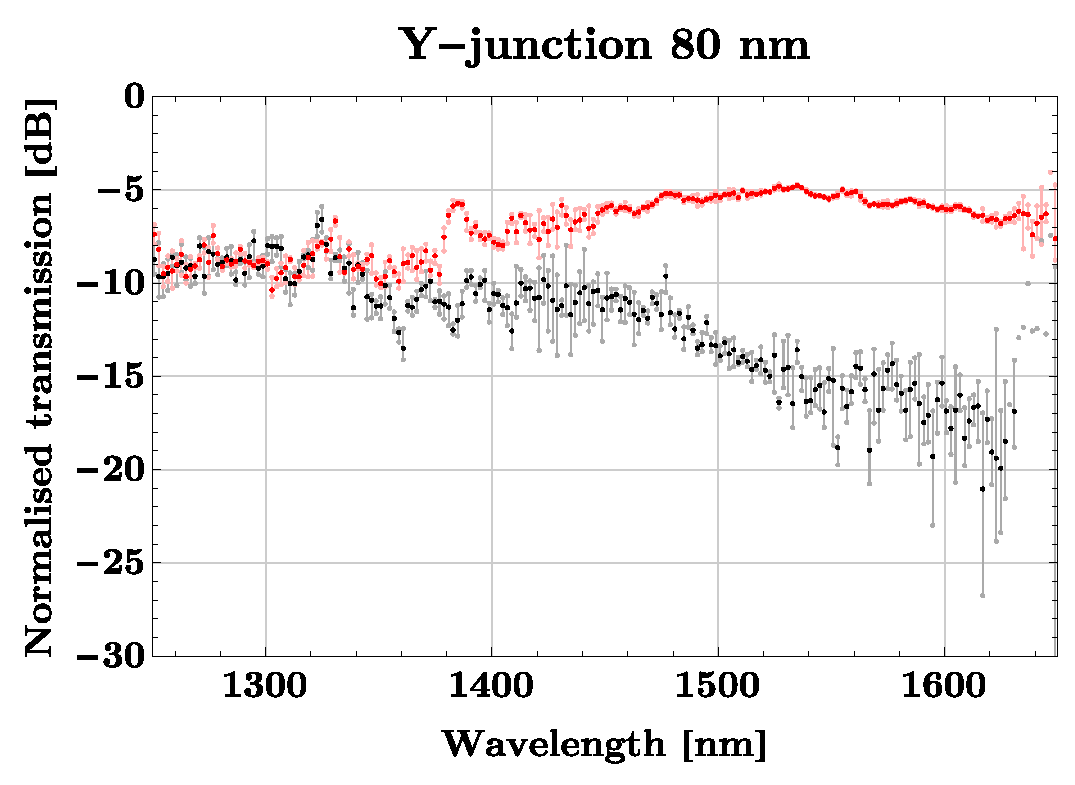
\includegraphics[width=1.0\textwidth]
        {fig/Kilde2Multimeter/yjunc80multimeterconcatenated.eps}
        \caption{Transmission through the Y-junction structure with feature size 80 nm.}
    \end{subfigure}
    \caption{Normalised transmission through fabricated structures. Black: Signal through upper output waveguide. Red: signal through lower output waveguide. The error bars mark maximum and minimum values obtained through 5-blocking (see the error bars subsection at page \pageref{sec:errorbars} for details). Measurements are obtained using the multimeter LEDs as light sources, see Table \ref{tablelightsources}.  The data are concatenated from two separate measurements; one measurement with the LED peaking at 1310 nm (data points in the interval  [1250, 1400] nm), one measurement with the LED peaking at 1550 nm (data points in the interval ]1400, 1650] nm).}
    \label{fig:transmissionkilde2conc}
    
\end{figure}

%

%Error bars are obtained through 5-blocking, see the Error Bars subsection (page \pageref{sec:errorbars}) for details.